\chapter{Egy frekvenciaváltó tervezése}

\paragraph{}

A napjainkban használt villamos gépeket az alábbiak szerint csoportosítjhatjuk:

\missingfigure{villamos gépek}

Amikor Tesla előállt az első háromfázisú indukciós motorral 1888-ban, nyilvánvalóvá vált, hogy az ilyen típusú gépek megbízhatóbbak és gazdaságosabbak tudnak lenni, mint az egyenáramú motorok. Jelentős hátrányuk azonban, hogy a vezérlésükhöz háromfázisú feszültséget kell előállítani, mely akkoriban cska egy szintén háromfázisú generátor segítségével volt megoldható. Manapság a háromfázisú teljesítmény a villamos hálózatnak köszönhetően rendelkezésre áll, azonban még így is vet fel prooblémákat ezen motorok üzemeltetése.

A frekvenciaváltó egy olyan eszköz mely váltakozó áramú bemenetből váltakozó áramú kimenetet állít elő, mint ahogy a neve is mutatja, más frekvenciával vagy akár feszültséggel, mint a bemenet. Erre azért van szükség, mert a meghajtani kívánt folyamatnak nagyon valószínű, hogy más igényei vannak, mint amit a hálózat önmagában képes biztosítani. Értem ez alatt azt, hogy közvetlen összeköttetés esetén a motorunk $50\ Hz-el$, vagy ennek egész számú hányadosával tudna forogni, illetve ennek a paraméter a befolyásolása fizikailag csak a motor módosításával lehetséges. Természetesen mint az ipar és az élet minden szegmensében itt is célunk a feladat minél hatékonyabb végrehajtása. A világon a teljes villamosenergia felhasználás mint egy $25\ \%-$-át adják a villamos hajtások és ez a szám folyamatosan nő (pl. az elektromos közlekedés térnyerésével). Az igény tehát nyilvánvaló ezeknek az eszközöknek a folyamatos fejlesztésére.

\begin{figure}[!h]
	\centering
	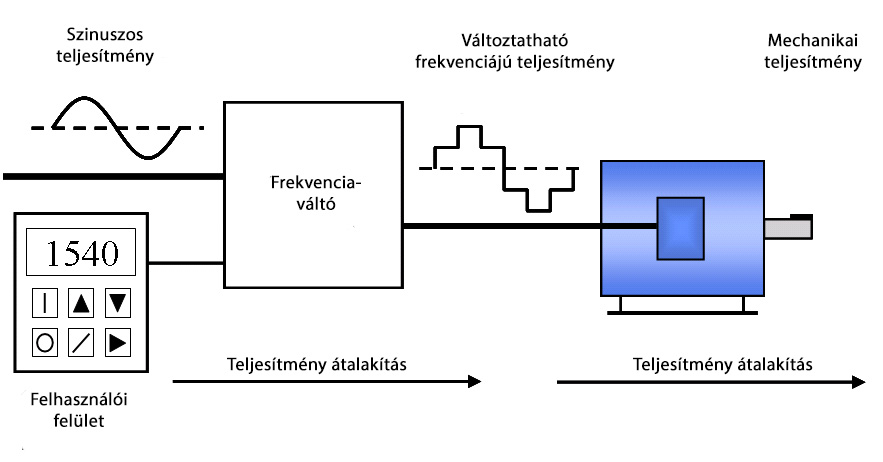
\includegraphics[width = 0.8\textwidth]{figures/VFD_System.jpg}
	\caption{A frekvenciaváltó szerepe} 
	\label{fig:vfd_system}
\end{figure}

Az eszköz feladatát jól összefoglalja \aref{fig:vfd_system} ábra. A hálózatból érkező teljesítményt, a felhasználó által megadott paraméterekkel átalakítjuk, majd a terhelő gépet meghajtuk vele. A modern hajtások ennél jóval szofisztikáltabb működésre is képesek, gondoljunk itt akár távfelügyeletre, identifikációra, vagy esetleg akár vezeték nélküli hozzáférésre.

\paragraph{}
A korábban az ilyen teljesítmény átalakítási feladatokat elektromechanikus berendezésekkel oldották meg, nevezetesen egy motor és generátor párral, ahol is a megfelelő póluspár arány kiválasztásával a frekvenciát módosítani lehetett. Amennyiben szükséges volt feszültségmódosítás is, megfelelő áttételű transzformátor segítségével valósították meg. Ennek a megoldásnak hátránya a nagy teljesítmény esetén nagy méretű villamos gép, ennek megfelelően a kicsi teljesítménysűrűség. A megbízhatóságot csökkenti a mozgó alaktrészek jelenléte és folyamatos igénybevétele, illetve a nagy forgó tömeg is hordoz magában veszélyeket. Ezt követően megjelentek a vákumcsöves eszközök, azonban az igazi áttörést a teljesítményelektronikai félvezető elemek megjelenése okozta.

Ezek a modern eszközök már tartalmaznak mozgó alakrészt (feltéve persze, hogy a reléket és kontaktorokat nem számmítjuk). A félvezető technológia fejlődésével egyre nagyobb és nagyobb teljesítménysűrűségeket tudunk elérni.

\begin{figure}[!h]
	\centering
	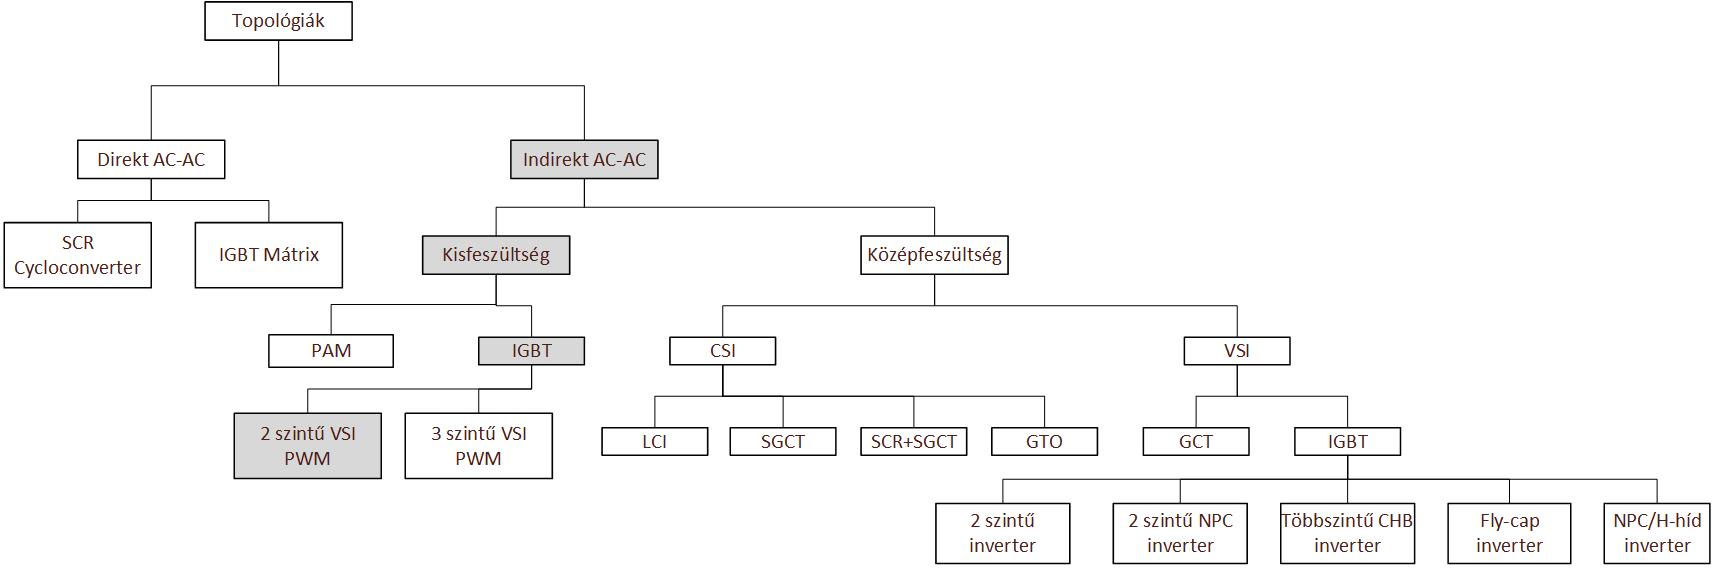
\includegraphics[width = \textwidth]{figures/topologies.jpg}
	\caption{A frekvenciaváltó szerepe} 
	\label{fig:topologies}
\end{figure}

\Aref{fig:topologies} ábrán láthatjuk a napjainkban elterjedt inverter típusokat. Az ábrában szürkével kiemeltem a Hyundai által fejlesztett típust.

\section{Termék specifikáció}

A Hyundai által jelenleg fejlesztett frekvenciaváltó család kis feszültségű, általános célú PWM vezérlet IGBT kapcsolóelemű 2 szintű inverteres frekvenciaváltó, passzív front-end-el, azaz a hálózatra nem tud visszatáplálni. \Aref{fig:family} táblázatban látható a jelenleg fejlesztett termékcsalád.

\begin{table}[]
\centering
\begin{tabular}{|c|c|c|c|l}
\cline{1-4}
\textbf{Név} & \textbf{Teljesítmény (kW)} & \textbf{Áram (A)} & \textbf{Tömeg (kg)} &  \\ \cline{1-4}
\multirow{4}{*}{\textbf{FR1}} & 0,55 & 3,7 & \multirow{4}{*}{6} &  \\ \cline{2-3}
 & 0,75 & 4,8 &  &  \\ \cline{2-3}
 & 1,1 & 6,6 &  &  \\ \cline{2-3}
 & 1,5 & 8 &  &  \\ \cline{1-4}
\multirow{3}{*}{\textbf{FR2}} & 2,2 & 11 & \multirow{3}{*}{10} &  \\ \cline{2-3}
 & 3,7 & 18 &  &  \\ \cline{2-3}
 & 5,5 & 25 &  &  \\ \cline{1-4}
\multirow{2}{*}{\textbf{FR3}} & 7,5 & 31 & \multirow{2}{*}{20} &  \\ \cline{2-3}
 & 11 & 48 &  &  \\ \cline{1-4}
\multirow{3}{*}{\textbf{FR4}} & 15 & 62 & \multirow{3}{*}{37,5} &  \\ \cline{2-3}
 & 18,5 & 75 &  &  \\ \cline{2-3}
 & 22 & 88 &  &  \\ \cline{1-4}
\multirow{3}{*}{\textbf{FR5}} & 30 & 114 & \multirow{3}{*}{66} &  \\ \cline{2-3}
 & 37 & 140 &  &  \\ \cline{2-3}
 & 45 & 170 &  &  \\ \cline{1-4}
\multirow{2}{*}{\textbf{FR6}} & 55 & 211 & \multirow{2}{*}{108} &  \\ \cline{2-3}
 & 75 & 261 &  &  \\ \cline{1-4}
\end{tabular}
\caption{A fejlesztés alatt álló termékpaletta}
\label{fig:family}
\end{table}

Azt, hogy a termék milyen széles területét lefedi az iparnak, jól jellemzi, hogy az ezt leíró dokmentum 52 különböző tételt különböztet meg. A teljesség igénye nélkül a felvevő piac néhány szelete:

\begin{itemize}
	\item{Nagyfeszültségű légkondícionálók}
	\item{Élelmiszeripar}
	\item{Textilipar}
	\item{Szállítószalagok}
	\item{Csomagolás és cimkézés}
	\item{Nyomtatás}
	\item{Gépi megmunkálás}
	\item{Autóipar}
\end{itemize}

A hardveres funkcionalitás nagyjából megegyezeik minden esetben, az igazán nagy különbség az egyes területek között a szoftver funkcionalitásában van. Egy szállítószalag esetében fontos a pontos fordulatszám tartása, vagy a pontos pozíció beállítása, míg más felhsználás esetében a potos nyomatékszabályozás lehet fontos, ilyen lehet pl. a villamos vontatás.

Amennyiben külön nincsen jelölve, a dolgozat a továbbiakban az FR1 kódjelű, legkisebb frekvenciaváltóra hivatkozik a példák esetében.

\section{Az eszköz felépítése}

\paragraph{}
A frekvenciaváltó egyenirányítja a bejövő hálózati feszültséget, egy köztes energiatárolóban, az ún. \emph{DC-link} kondenzátorban tárol némi energiát, hogy a feszültség lengésést alacsonyan tartsa, majd egy kimeneti inverterrel előállítja a szükséges jelalakot. Ezt a vázlatot láthatjuk \aref{fig:vfd_schema} ábrán, kiemelve a hálózatot modellező ellenállást és induktivitást.

\begin{figure}[h]
	\centering
	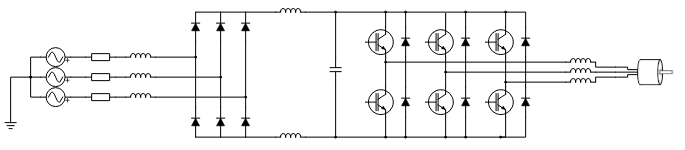
\includegraphics[width = \textwidth]{figures/VFDschematic_choke.png}
	\caption{A frekvenciaváltó egyszerű felépítése} 
	\label{fig:vfd_schema}
\end{figure}

Itt természetesen csak egy vázlatos ábrázolás látató, ezen nem szerepelnek a megható elektronikák, a vezérlés, a mérések, és még sok más. Jól látható azonban, hogy a folyamatra egyedül a félhidak vezérlésével tudunk hatni. A Frame 1-ben a kimeneti IGBT-k és diódák egy tokban vannak, egy modulban. 




\section{A szükséges kompetenciák}
\section{A fejlesztés folyamata}
